
\documentclass[runningheads]{llncs}
%
\usepackage{graphicx}
% Used for displaying a sample figure. If possible, figure files should
% be included in EPS format.
%
% If you use the hyperref package, please uncomment the following line
% to display URLs in blue roman font according to Springer's eBook style:
% \renewcommand\UrlFont{\color{blue}\rmfamily}

\begin{document}
%
\title{Norwegian Correspondences and\\Linked Open Data}
%
%\titlerunning{Abbreviated paper title}
% If the paper title is too long for the running head, you can set
% an abbreviated paper title here
%
\author{Authors}
%
\authorrunning{Author et al.}
% First names are abbreviated in the running head.
% If there are more than two authors, 'et al.' is used.
%
\institute{Organisations}

%
\maketitle              % typeset the header of the contribution
%
\begin{abstract}
The project \textit{Norwegian Correspondences} aims to link individual letters and other correspondence media not only to each other but to correspondences accross entire Norway, Europe and beyond. It uses the CorrespSearch infrastructure, which employs Linked
Open Data standards. Correspondence metadata from digitized letters, digital and printed scholarly editions is delivered in the Correspondence Metatdata Interchange Format (CMIF). Via the web interface, data can be easily searched\textemdash or queried via an open API. 

\keywords{Correspondence \and Cultural Heritage Institutions \and Linked Data  \and Collaboration.}
\end{abstract}
%
\section{About the Project}
The National Library of Norway has a substantial amount of private
historical correspondences in its
holdings,\footnote{The manuscript catalogue contains almost 200.000 letters.} some of them are scholarly
edited and published, either in printed editions or in digital form. In
addition, other Norwegian cultural heritage institutions, like the Munch
Museum,\footnote{The Munch Museum holds 8.802 letters to and from Edvard Munch.} but also the university
libraries of The Arctic University of
Norway and the University of
Bergen\footnote{The Section for Special Collections, holds
ca. 600 separate collections of letters.} and the Gunnerus Library at
the Norwegian University of Science and
Technology, hold significant
collections of letters and are preparing digital editions of letters and
correspondences of key figures of Norwegian public and academic life.
Yet, all these correspondence projects lead a solitary existence--hidden
either in editions of single authors or as digitized collections or
individual pieces on institutional servers.

As a dialogical genre by nature, the full potential of letters and other correspondance material lies in the connection of the individuals writing and receiving letters, postcards, and telegrams--at a specific time and from and to a specific place. But because the collections of letters and individual pieces of a correspondence are historically
distributed wide and far in regards to geography and institution, there rarely exist links between them. Thus research on correspondence
networks that existed in Norway, the Nordic Countries--and beyond, to Europe and the rest of the world--as well as research on the letter as the main means of written communication for centuries is almost
impossible.

The project \textit{Norwegian Correspondences} (\textit{NorKorr}, from Norwegian \textit{Norske korrespondanser}) aims to link these individual letters and similar materials not only to each other but to correspondences in
entire Norway, Europe and beyond by use of the CorrespSearch~\cite{ref_url9}
infrastructure. CorrespSearch is both an infrastructure for connecting correspondences accross editions and collections making use of Linked Open Data (building on VIAF and GeoNames among other openly available datasets) and a web service that aggregates specific correspondence
metadata from digital and printed scholarly
editions.~\cite{ref_article} These data can be easily
searched via the CorrespSearch web interface or queried via their open API. By integrating Norwegian correspondences in the corpus of letters that already exists on CorrespSearch, they will become visible as part of a greater international network of letters and allow for a
macroscopic view on the correspondence networks that existed throughout the centuries.

\subsection{Aims}
The aim of the NorKorr project is to aggregate and provide
correspondence metadata from Norwegian editions of correspondences from
different projects, institutions and collections in a format that can be
ingested by CorrespSearch. The metadata in question are comprised of (1)
names of writer and receiver of the letter (preferably with reference to
the Virtual International Authority File
VIAF).~\cite{ref_url3} (2) A unique identifier for each
letter, usually in form of a URN. (3) Optionally, the places letters
were sent from and to (preferably with reference to
GeoNames).~\cite{ref_url4} (4) Optionally, the date of
writing (in the ISO standard).~\cite{ref_url5} The final
product will be a large set of metadata for Norwegian correspondences
under a Creative Commons 4.0 License in the 
Correspondence
Metadata Interchange Format (CMIF) standard~\cite{ref_url10} and an open workflow for
(semi-)automatically creating and delivering CMIF-compliant
correspondence metadata from future editions to the
CorrespSearch web service.

In addition to aggregating the metadata from digital and printed
(scholarly) editions, \textit{NorKorr} aims to incorporate all digitized
correspondence material. This means that all manuscript and private
archive collections throughout Norway which have undergone or will
undergo digitization and assign individual URNs to each letter together
with a minimum of metadata (often derived from manuscript catalogues)
will be interconnected.~\cite{ref_proc} At the
present, CorrespSearch doesn't incorporate material that is not
(scholarly) edited in either digital or printed format. NorKorr will,
however, collect all correspondence metadata regardless and map it on
the CMIF standard using the URNs as persistant identifiers for
individual letters. It will thus be possible to use the existing
infrastructure that CorrespSearch provides to connect material in almost
all forms: scholarly edited, printed or digital, and digitized.

We see this expansion to be an important step towards making digital
collections accessible and searchable cross-institutionally, a feature
that is usually prevented by mutually incommensurable in-house
solutions regarding encoding standards, cataloguing methods and metadata
standards. In addition, because it is commonly only a small and often
strongly canonised selection of authors, musicians, artists and
academics whose letters are deemed worthy of a scholarly edition, the
picture we have of Norwegian correspondence networks and Norwegian
cultural contacts with the other Nordic countries and the rest of the
world is strongly biased and non-representative. NorKorr is able to
include correspondence material regardless of language, time period,
social class, gender, and nationality.
\subsection{Status Quo}\label{status-quo}
\subsubsection{Scope}\label{scope}
We propose to present a collaborative poster where we focus
on five cases of correspondence collections at Norwegian cultural
heritage institutions. For the cases, we decided to be as diverse and
multifaceted as possible. We will describe the collections of letters of
each contributing institution and the specific challenges each of these
collections poses in regard to content, technology and workflows we
have established for connecting our correspondences.

\subsubsection{Case 1 -- Letters from Norwegian Writer and Feminist
Camilla Collett
(1813-1895)}
The National Library of Norway has approximately 1.000 letters written
by  Norwegian author Camilla Collett in its manuscript
collection. More than half of these letters have never been published.
Collett's handwriting is difficult to read and there has been little
research on them. We want to make the letters more
available by transcribing, encoding and publishing them. One of the
publications is a digital edition containing ca. 50 letters
written by Collett between 1841–1851. The edition is part of the
library's source edition series NB kilder, published on the e-book
website Bokselskap.~\cite{url_boks}

\begin{figure}
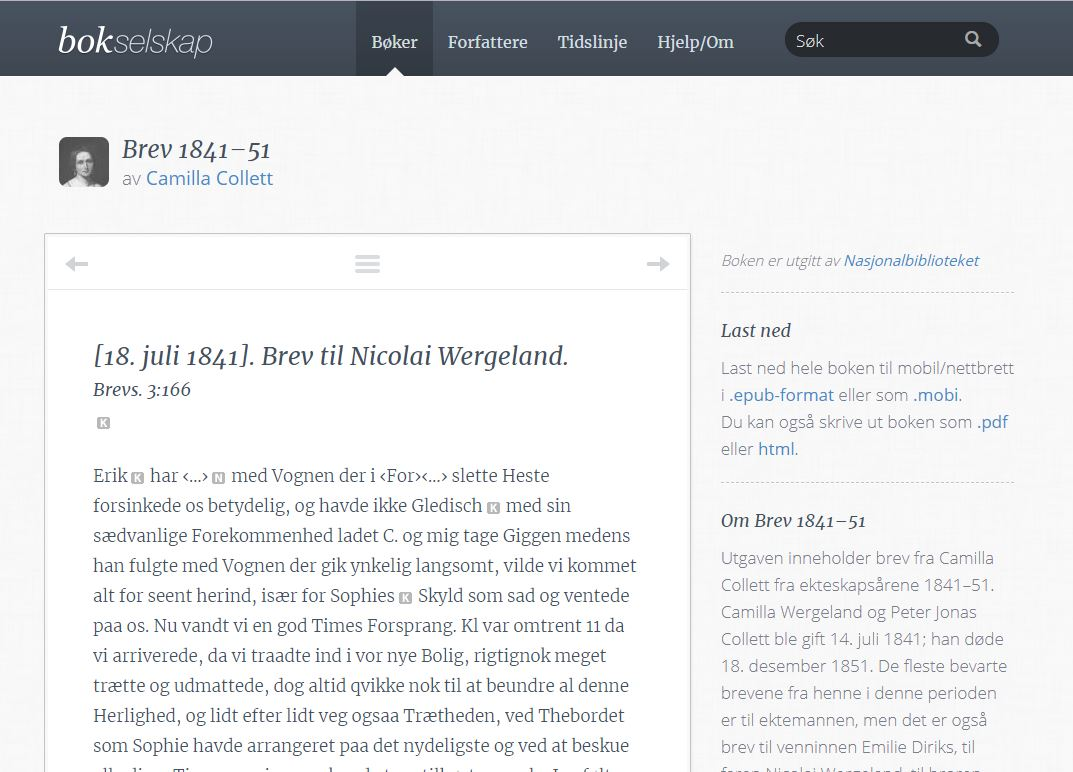
\includegraphics[width=\textwidth]{CC_BS.jpg}
\caption{Screenshot from the digital edition} \label{fig1}
\end{figure}

The letters are encoded in TEI P5 XML. To get the letters registered and
integrated into the CorrespSearch web service we create a CMIF file
based on the metadata already recorded in the \texttt{correspDesc}
element in our XML files.

\begin{figure}
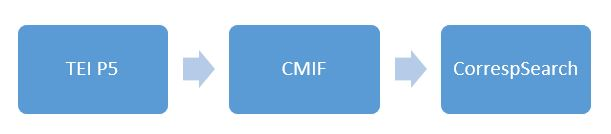
\includegraphics[width=\textwidth]{TEI-CMIF.jpg}
\caption{The workflow} \label{fig2}
\end{figure}

\begin{figure}
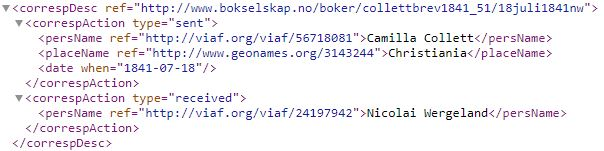
\includegraphics[width=\textwidth]{correspDesc.jpg}
\caption{Screenshot from the CMIF file} \label{fig3}
\end{figure}

\begin{figure}
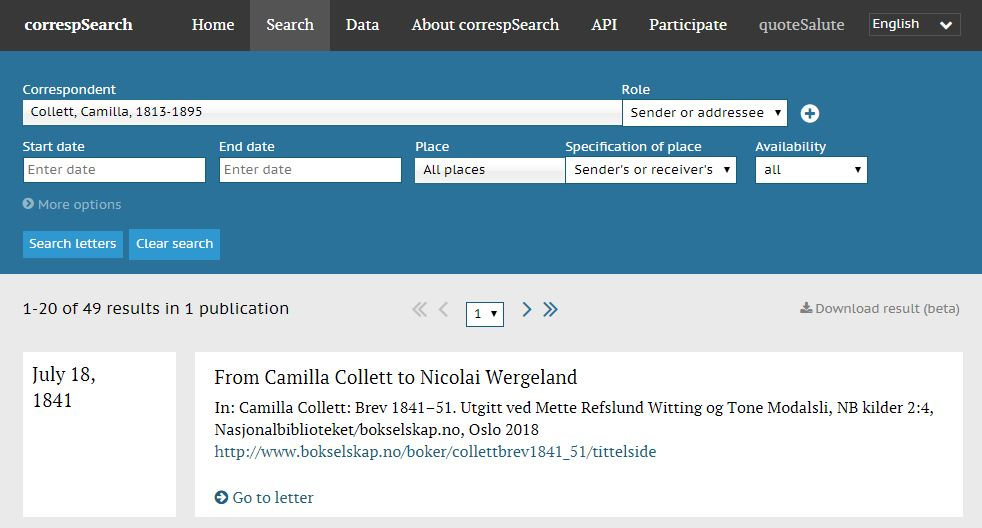
\includegraphics[width=\textwidth]{CC_CS.jpg}
\caption{Screenshot from the CorrespSearch web service, where the Collett data is searchable} \label{fig4}
\end{figure}

\subsubsection{Case 2 -- Letters to and from Norwegian Artist Edvard
Munch (1863-1944)}
Norwegian artist Edvard Munch's correspondence with family and friends,
and with assistants, patrons, collectors, art dealers, printers,
newspaper and magazine editors, artists, writers, art historians,
exhibition organisers, gallery owners, shipping companies, and more,
comprises more than 10.000 known letters and letter drafts.

Among the more than 800 senders and 400 recipients currently in our
online registers~\cite{ref_emunch} are well-known names that
are easy to connect to authoritative identifiers, but also many that
aren't. Among those not present in authority registers are Munch's
family and some of the friends he most eagerly exchanged letters with as
well as other important people and institutions. The letters are written
in Norwegian, German, Danish, Swedish and French as well as the odd
occurrence of English, Italian, Spanish, Polish and Czech. The letters
span 70 years, from 1874 to 1944, representing hundreds of handwriting
styles and many types of letters. Metadata are partially incomplete;
Munch himself didn't always bother adding date and place to letters, and
envelopes are often missing, so analysing the content is necessary to
discover when and where a letter was written and whereto it was sent.

\begin{figure}
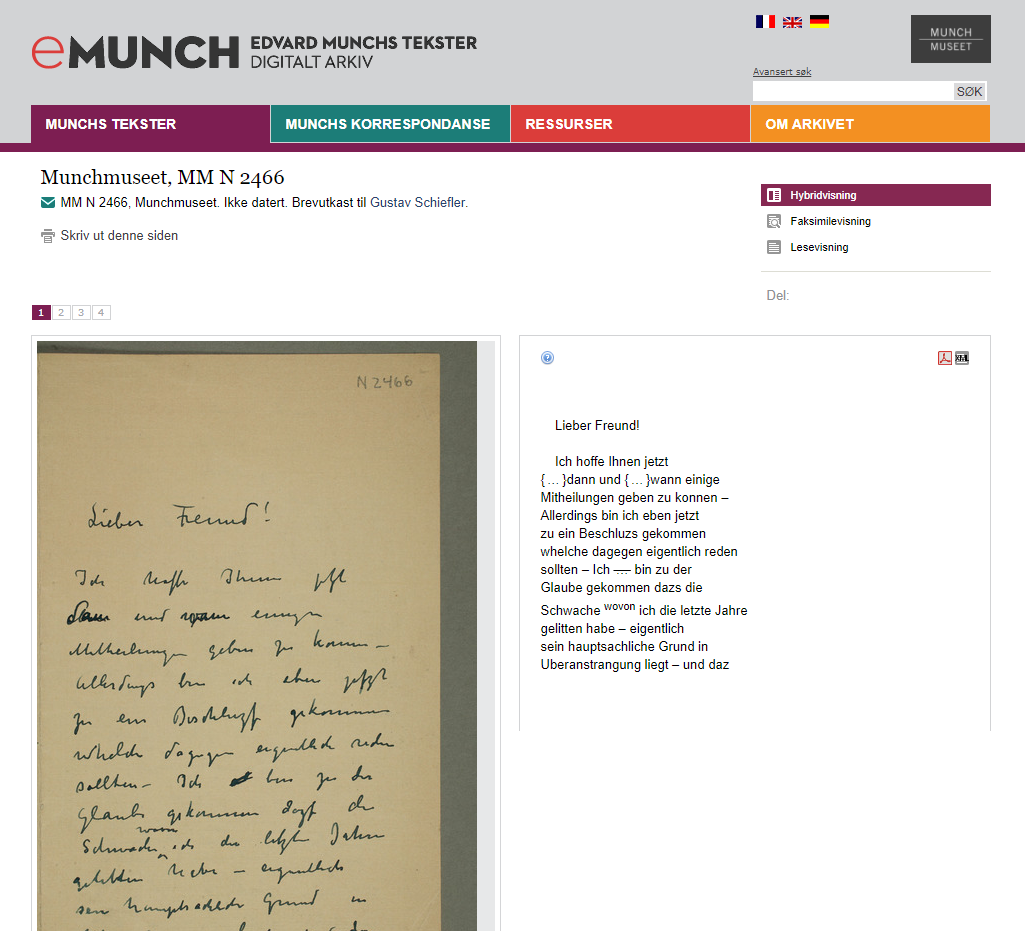
\includegraphics[width=\textwidth]{emunch.png}
\caption{Screenshot from the digital edition} \label{fig5}
\end{figure}

\subsubsection{Case 3 -- Correspondence Collections from the University Library at the Norwegian University of Science and Technology}
The following four letter collections highlight the special collections
of NTNU University Library through their international correspondence,
thus showing their importance for adding them to a common database.

\begin{figure}
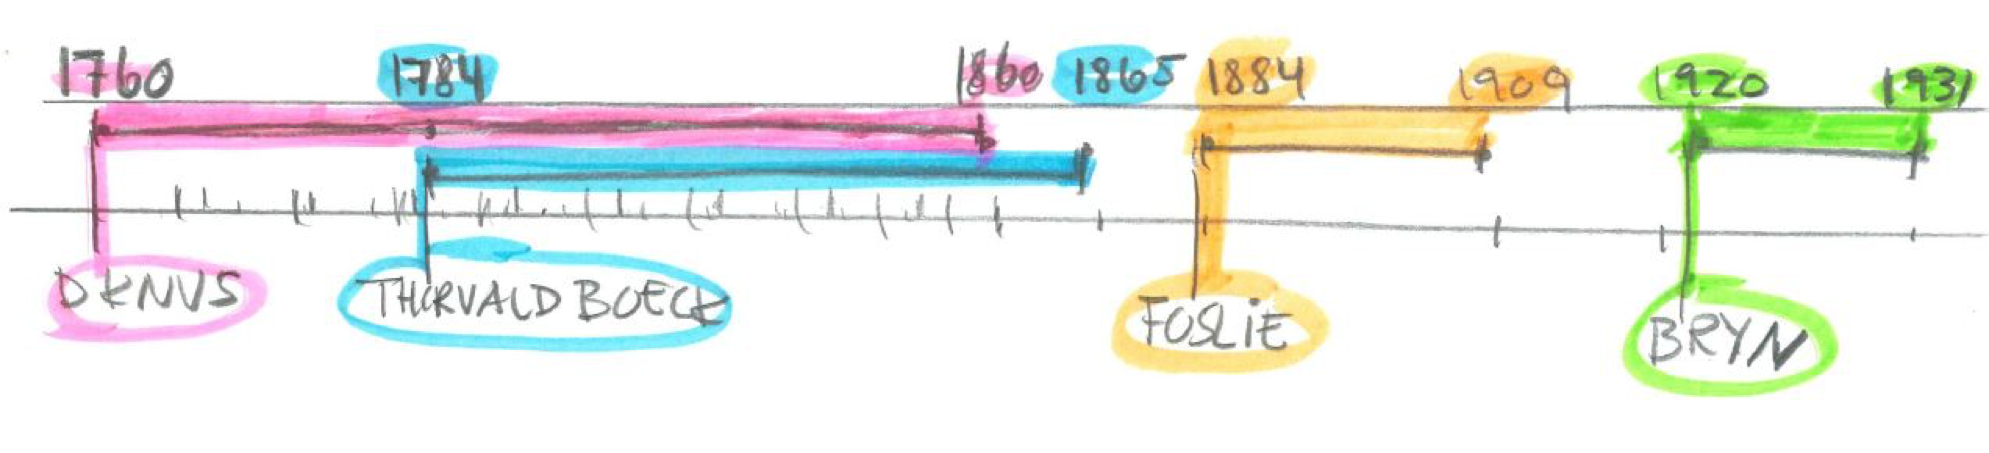
\includegraphics[width=\textwidth]{NTNU_case_sketch.png}
\caption{Timeline for Collections from NTNU University Library} \label{fig6}
\end{figure}

\textbf{The Royal Norwegian Society for Sciences and Letters} consists of 3.738 letters from the first 100 years (1760-1860) of its existence, among them letters from Carl von Linné, Artur Schopenhauer, Henrik Wergeland, Ivar Aasen, and many other known people who played a part in culture and science in that time.
\textbf{Thorvald Boeck (1835-1901)} was a famous collector and known for assembling what was the largest private library of its time in Norway. The collection of 2.294 letters from 1784-1865 are diverse and consist among others of Royal senders and other famous persons. 
\textbf{Mikael Heggelund Foslie (1855-1909)} was one of the most important international researchers on the systematics of non-geniculate coralline red algae at the turn of the 19th century. From 1892 until his death he worked in Trondheim as a curator at the Museum of the Royal Norwegian Society for Sciences and Letters (DKNVS). His correspondence is an example of a worldwide scientific communication and discussion and the exchange of species among scientists. This  collection of letters on botanical issues from 1884-1909 consists of 1.963 letters~\cite{ref_algae}
\textbf{Halfdan Bryn (1864-1933)} was a Norwegian physician and physical anthropologist. As an army doctor, Bryn had opportunity to study men from different parts of Norway and this inspired him to do his research. The collection consists of 830 letters from 1920-1931.~\cite{ref_halfdan}

\subsubsection{Case 4 -- The Letter Collections at University of Bergen Library}
By focusing on three disparate collections of letters from the Section
for Special Collections, we wish to show the value and potential of
linking and contextualizing these collections in a correspondence
database.

The first collection, \textbf{Ms 790}~\cite{ref_url6},
actively collected by the Bank Officer O.J. Larsen, contains ca. 2.100 letters written by Norwegian and European celebrities, from Camilla
Collett and Edvard Munch to Napoleon, Goethe and Lord Byron. As a
curated collection, the letters defy a normal correspondence
pattern. However, within a correspondence database new links to similar
collections and related letters can elucidate the original correspondence.

The second collection, \textbf{Ms 2083}~\cite{ref_url7},
contains around 350 letters sent to the physician, leprosy scientist,
zoologist, and director at Bergens Museum, D.C. Danielssen (1815-1894).
This fascinating collection reveals the wide-ranging exchange and
collaboration of scientific research and ideas between Danielssen and
scientists in Scandinavia and Europe.

Finally, \textbf{Ms 2155}~\cite{ref_url8}, the Mons Flaesland
Collection, is a private collection, containing ca. 950 family letters
from the period 1895-1930. The collection describes everyday life,
relations and destinies through three generations of detailed family
letters. This uniquely preserved collection is equally important as a
reflection of social conditions and class distinctions.

\begin{figure}
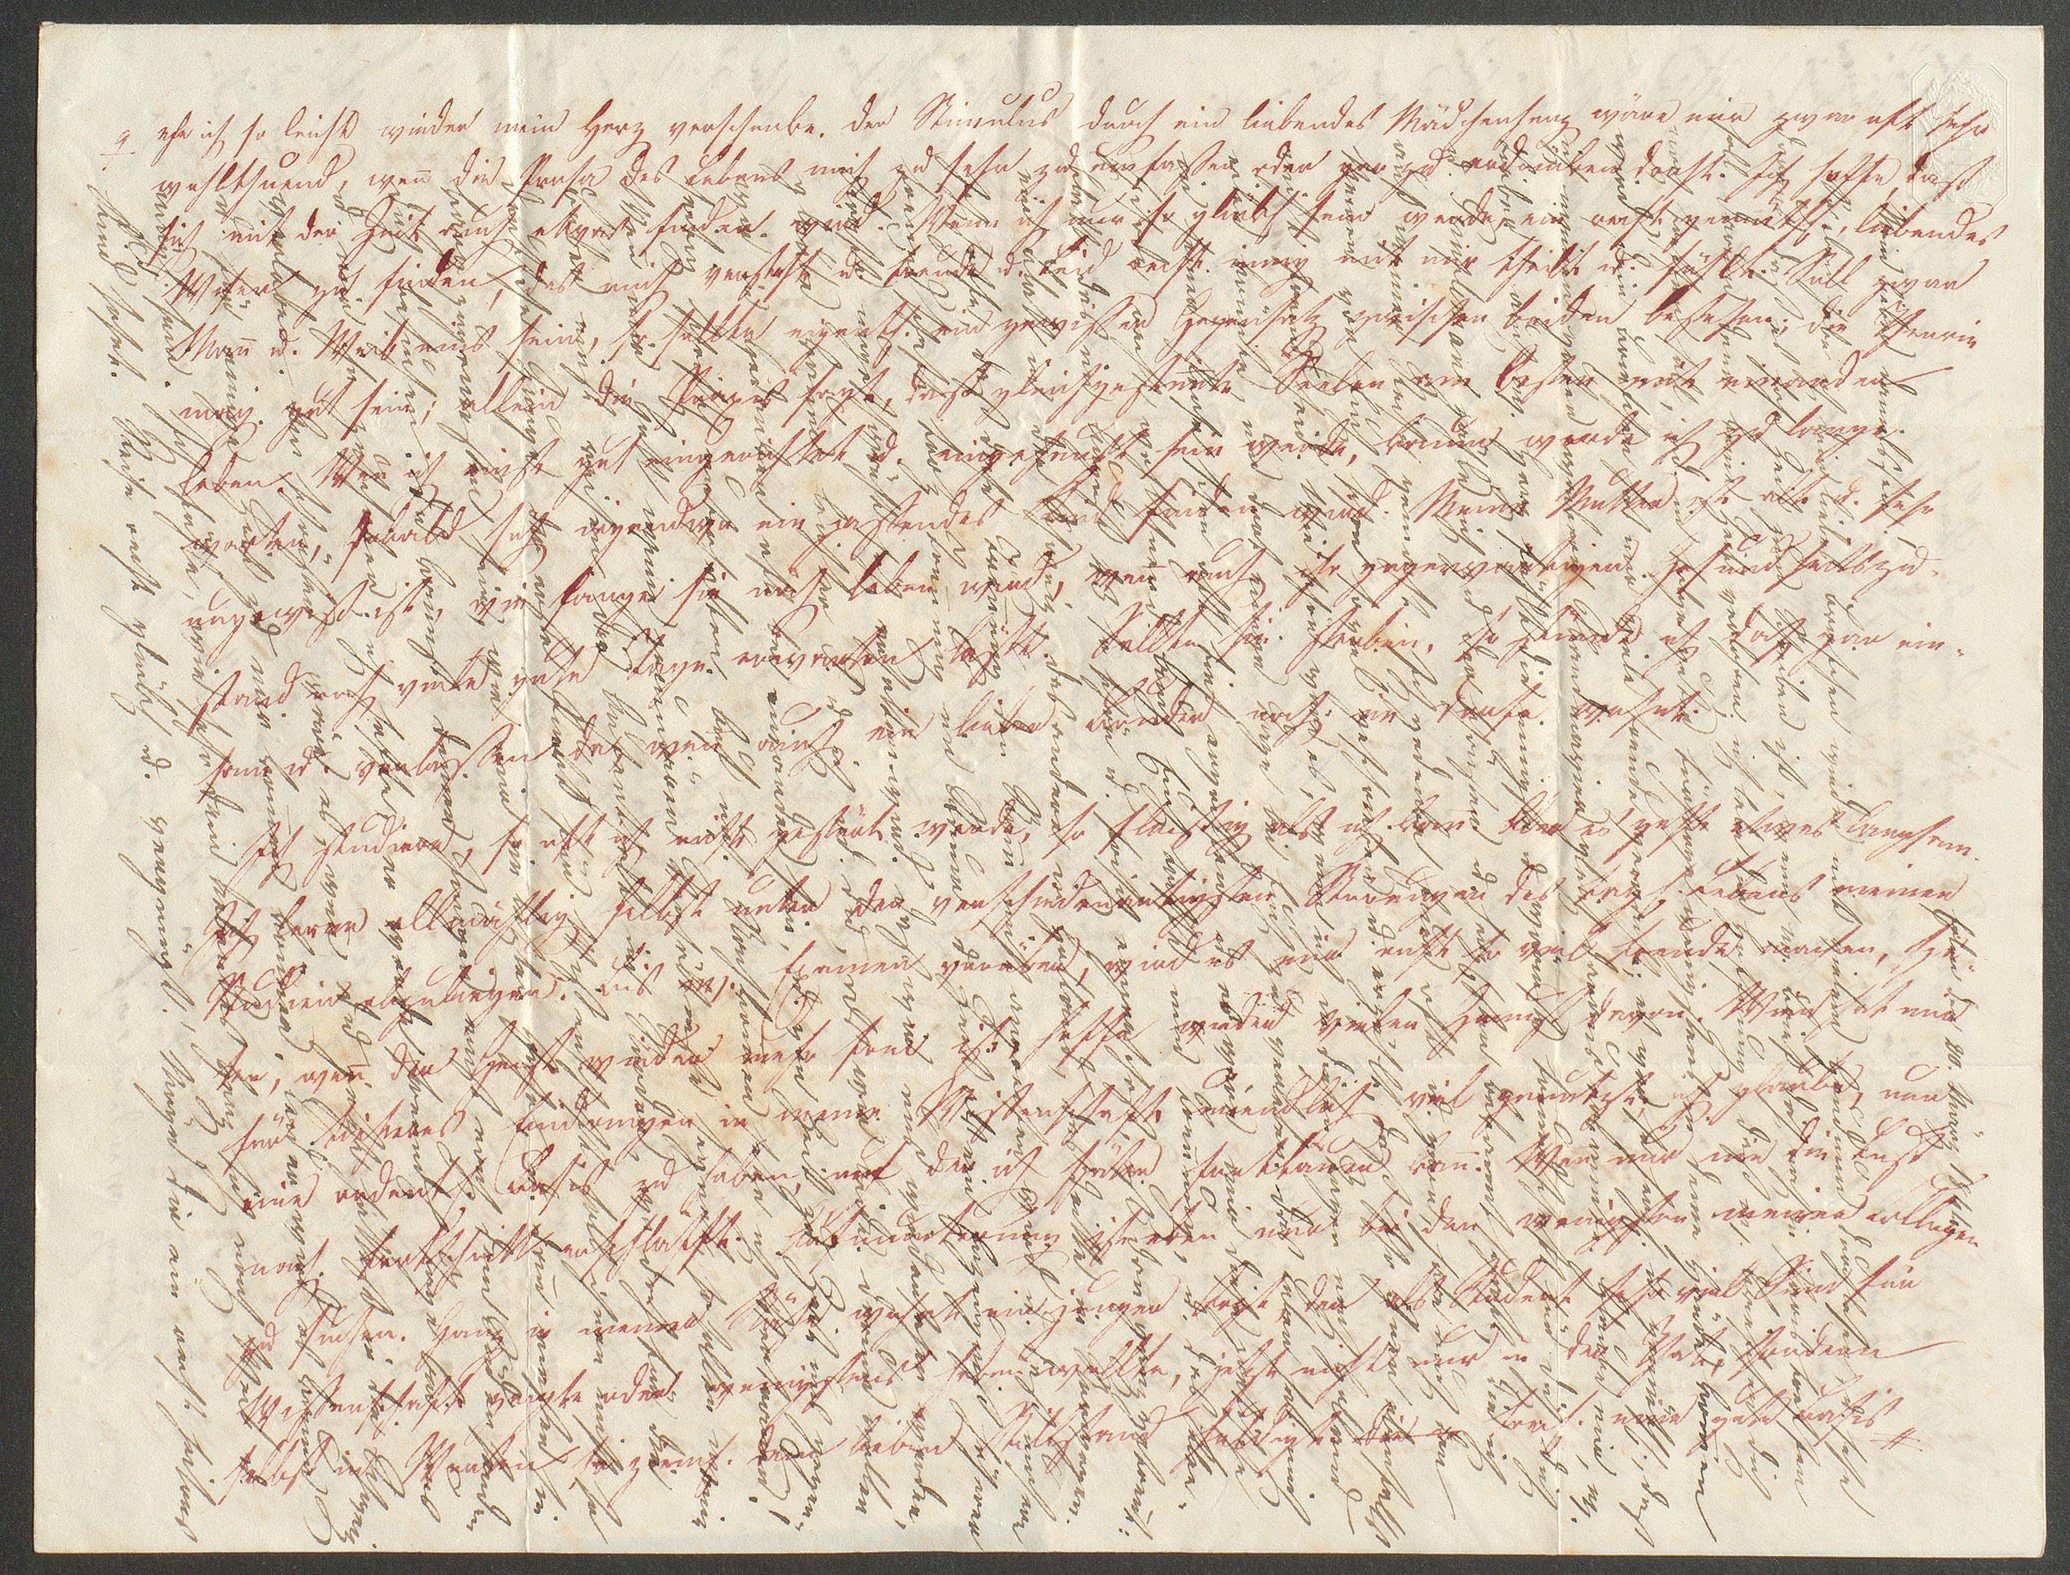
\includegraphics[width=\textwidth]{ubb-ms-2083-b-1-09_Letter_to_DCDanielssen.jpg}
\caption{Dated 20th of March 1844 this crossed letter from Ms 2083 was written by Diethelm in Frauenfeld and sent to D.C. Danielssen in Bergen.} \label{fig7}
\end{figure}

\subsubsection{Case 5 -- Letters from Norwegian philologist and ethnographer Just Knud Qvigstad (1853-1957)}
Just Knud Qvigstad was en expert on Sami language and culture
(lappologist). He worked as the headmaster of the Tromsø Teacher
Training College, which is one of the predecessors of UiT The Arctic
University of Norway.

During several decades, Qvigstad was involved in an extensive
correspondence with other experts on Sami from Norway, Scandinavia, and
other countries. Some of Qvigstad's letters were digitized, transcribed,
and published online as part of the Documentation
Project~\cite{ref_dokpro} in the early 1990s:
\begin{itemize}
\tightlist
\item
  Qvigstad to Magnus Olsen (1909-1956) (65 letters), held at the
  National Library of Norway.
\item
  Qvigstad to K. B. Wiklund (1891-1936) (96 letters), held at Uppsala
  University Library.
\item
  Qvigstad to Emil N. Setälä (1887-1935) (96 letters), held at the
  National Archives of Finland, prof. Setälä's private archive.
\end{itemize}

\begin{figure}
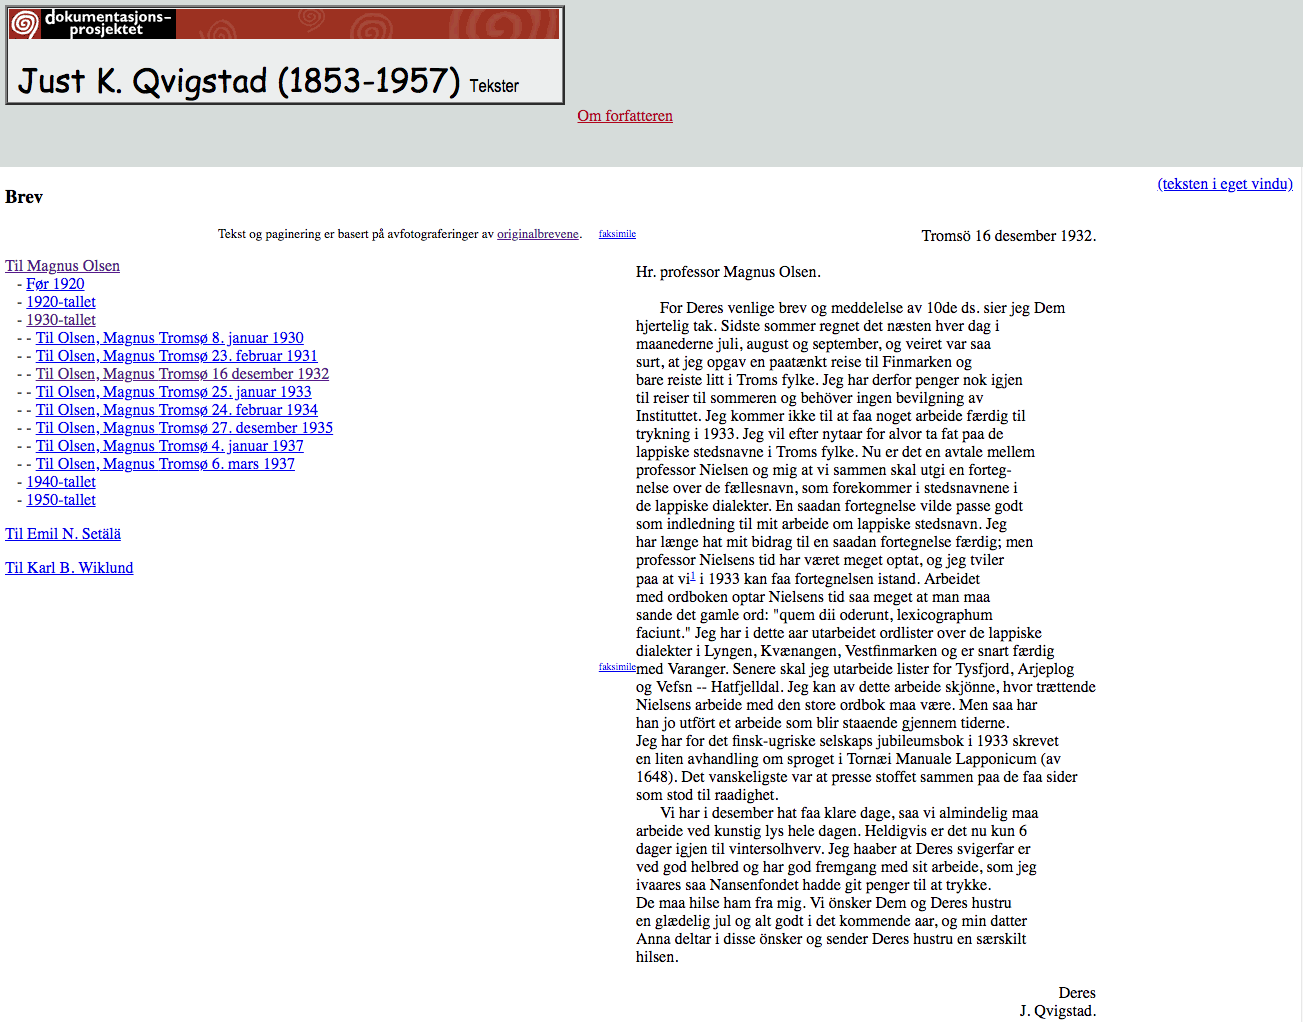
\includegraphics[width=\textwidth]{qvigstad_dokprosjekt_snapshot.png}
\caption{Screenshot of the early digital scholarly edition of Qvigstad's letters} \label{fig8}
\end{figure}
More than 20 years have passed since the publication of these letters.
The aim of the project \textbf{Qvigstad's Correspondence 2.0} at the UiT
University Library is to re-edit the letters according to the
requirements to a modern digital scholarly edition, including the
following enhancements:

\begin{itemize}
\tightlist
\item
  Providing high resolution tif/jpg facsimile images
\item
  SGML to XML/TEI P5 conversion of the transcription
\item
  Embedding in virtual research environment for humanities: TextGrid
\item
  Up-to-date web interface
\end{itemize}

In addition, the letters to Sophus Bugge (1833-1907) will be included.
In collaboration with the National Library of Norway, a selection of
letters will be published as a reader-friendly edition in NB kilder.

\subsubsection{Project Website}\label{project-website}

The project \textit{NorKorr} is collectively developed on GitHub \textit{in plain
view}. It is open for collaborators from all Norwegian cultural heritage
institions (ALM sector), the universities and other research
institutions as well as other organisations who hold collections of
correspondence material. We document our code and share it under the
Creative Commons Attribution 4.0 License. We build on the work shared by
the CorrespSearch team, the TEI Correspondence SIG and individual
researchers and developers on GitHub.

\begin{thebibliography}{8}

\bibitem{ref_url9}
CorrespSearch Website \url{https://correspsearch.net/index.xql}
Last accessed 18 Oct 2018

\bibitem{ref_article}
Dumont, S.: CorrespSearch - Connecting Scholarly Editions of Letters. Journal of the Text Encoding Initiative \textbf{10}, (2016)

\bibitem{ref_url3}
VIAF Dataset \url{http://viaf.org/viaf/data/}
Last accessed 18 Oct 2018

\bibitem{ref_url4}
GeoNames \url{https://www.geonames.org/}
Last accessed 18 Oct 2018

\bibitem{ref_url5}
ISO 8601 Standard \url{https://www.iso.org/standard/40874.html}
Last accessed 18 Oct 2018

\bibitem{ref_url10}
CMIF Standard Documentation \url{https://github.com/TEI-Correspondence-SIG/CMIF}
Last accessed 18 Oct 2018

\bibitem{ref_proc}
Rettinghaus, K.: Semantic minimal retrospective digitization of edited correspondence. Poster. TEI2018 International Conference, Tokyo, 9-13 Sep 2018

\bibitem{url_boks}
\url{http://www.bokselskap.no/boker/collettbrev1841-51/tittelside}
% link is false! must be _ instead of -
Last accessed 18 Oct 2018

\bibitem{ref_emunch}
\url{https:/emunch.no/}
Last accessed 18 Oct 2018

\bibitem{ref_algae}
\url{https://www.ntnu.no/blogger/ub-spesialsamlinger/en/2017/03/23/coralline-algae-now-soon-online/}
Last accessed 18 Oct 2018

\bibitem{ref_halfdan}
\url{https://www.ntnu.no/blogger/ub-spesialsamlinger/2016/04/26/halfdan-bryns-korrespondanse-digitalisert/}
Last accessed 18 Oct 2018

\bibitem{ref_url6}
Collection MS 0790 \url{http://marcus.uib.no/instance/collection/ubb-ms-0790}
Last accessed 18 Oct 2018

\bibitem{ref_url7}
Collection MS 2083 \url{marcus.uib.no/instance/collection/ubb-ms-2083}
Last accessed 18 Oct 2018

\bibitem{ref_url8}
Collection MS 2155 \url{marcus.uib.no/instance/collection/ubb-ms-2155}
Last accessed 18 Oct 2018

\bibitem{ref_dokpro}
\url{https://www.dokpro.uio.no/qvigstad/ombrev.html}
Last accessed 18 Oct 2018

\end{thebibliography}
\end{document}
